
\clearpage
\section{Inferring Networks}

The following part describes the pipeline for generating spatial proximity networks out of honey bee tracking data. A node in the network is a bee. They are distinguished by IDs. Only bees are in the network who interact at least once with another bee.

undirected and weighted, aggregated networks\\

Two bees are associated (spatially close to each other), if their distance is minor to a \emph{maximum distance}. As everything is very close in a bee hive this value is hard to choose. Only this criteria is very week, meaning having a resolution of three frames per seconds results in interactions which could only last for $0.33$ seconds. So an additional parameter the \emph{minimum contact duration} is introduced, it is the minimum time they have to spend at least nearby to be called associated.

Taking the fragmentation of tracks into account, it is obvious that two bees could be nearby but not at the very same time, but slightly shifted. So the minimum contact duration would be too errow prone. To overcome this issue one could correct the bee tracks, by filling gaps of varius sizes and interpolating the position of that bee accordingly. This is rather time consuming for this amount of tracking data (TODO: naja so doll auch nicht) and also considering, that the tracking data is going to be improved in the future, then manipulating the raw data seems senseless. I rather perform a gap filling (maybe similar to binary dilation?) on the time series of pairs, but not on the bee tracks, because this is independent of the input data.

Edges are attributed with two parameters. The first one is the frequency of contacts, so how often they share a close position. The second parameter is the total duration of contact, how many time frames in total they spend close by.

\subsection{Network Pipeline}

The network pipeline takes as input a path to the bb-binary data and outputs a graph in graphML file format. The pipeline takes the following parameters:

\begin{itemize}
\item path to data
\item confidence in percent
\item gap size in frames - this is used to corret the time series of bee pairs
\item maximum distance in px - define what close means (spatial proximity)
\item minimum contact duration in frames - how many frames bees need to spend nearby
\item cutoff in percent - IDs with a number of total detections below X percent of the mean frequency are discarded 
\item start timestamp - start of network slice
\item window size in minutes - size of time window for aggregating the network
\item number of used CPUs for parallelization
\item year - calculate IDs and set camera setup for 2015 or 2016
\end{itemize}

The pipeline is parallelized on frame level, that means, each process gets a portion (frames for a timeinterval of five minutes) of the data and extracts interactions/edges. The main process adds everything up and creates a network.
The steps are the following:

\begin{enumerate}
\item \textbf{Filter detections by confidence}\\
For each of the four camera the detections are filtered by the confidence level.

\item \textbf{Simple stitching}\\
Each side of the hive consists of two cameras. 	The $x$-coordinates of each detection (of the right	cameras) is moved further to the right, also adding an offset of $2\times \texttt{maximum distance}$. So the left and the right detection of each side of the hive are move into one reference system.

\item \textbf{Syncronize Cameras}\\
For each side of the hive the cameras need to be syncronized. In the normal case the difference between consecutive frames should be about $0.332$~seconds, due to technical problem this value can be lower ($0.003$ ) and higher ($2.932$) at certain times. Cameras 3 and 2 and cameras 1 and 0 are matched, frames without a match are dropped (shorter number of frames, matchen, threshold $0.33/2$, minimum).

\item \textbf{Discard Detections with certain IDs}\\
All detections whos ID is in a list are keept, other detections are discarded. (see frequency filter)

\item \textbf{Extract close pairs}\\
For each side of the hive, all close pairs according to the maximum distance parameter are calculated and then joined together.

\item \textbf{Generate time series of bee pairs}\\
The data structure (frames and detection) is transformed to time series of bee pairs.

\item \textbf{Correct pair time series.}\\
The time series of bees are corrected by filling in the gaps of length \texttt{gap size}.

\item \textbf{Extract edges}\\
The edges and its attributes (frequency and duration) are extracted from the time series of bees using the minimum contact duration parameter. A sequence of at least X ones counts as one interaction. The frequency of those series adn the total duration (number of ones) are the attributes.


\end{enumerate}

\subsection{Pipeline Parameters}
For performing the network analysis, I chose the pipeline parameters as follows:

\begin{description}
\item[Confidence] As explained in section\ref{subsec:confidence}, the confidence is set to $95\%$.

\item[Maximum Distance] I chose the length of a bee body, according to \textcite{baracchi2014socio}, as the maximum distance between two bees (figure~\ref{fig:radius}). The average bee length of $212$px ($\pm 16$px)  was determinded by manually measuring the length of all bees ($n=337$) in four images (one for each camera, 21.07.2016, 03:00PM) using the tool ImageJ\footnote{\url{http://imagej.net/Welcome}; Last accessed: 22.02.2016}.

\item[Gap Size] The gap size is set to two frames. This value corresponds to the median gap length in the time series of pairs ($\texttt{mode}=1$, $\texttt{mean}=27$). [TODO: what dataset was used (95\% confidence, XXX\% cutOff, XXXpx maximal distance, date, camera)]

\item[Minimum Contact Duration] This is set to three frames (one second). This corresponds to~\textcite{mersch2013tracking}, they as well exclude interactions below one second. Looking at the frequency distribution of chains of ones ($1$, $11$, $111$, and so on) of the pair time series (after filling the gaps), then: $\texttt{mode}=1$, $\texttt{median}=2$ and $\texttt{mean}=4$. Three frames corresponds to $57\%$ of all chains, this seem to be reasonable. [TODO: what dataset was used (95\% confidence, XXX\% cutOff, XXXpx maximal distance, date, camera)]

\end{description}

\begin{figure}[htb]
	\centering
	\begin{subfigure}[b]{0.4\textwidth}
		\centering
		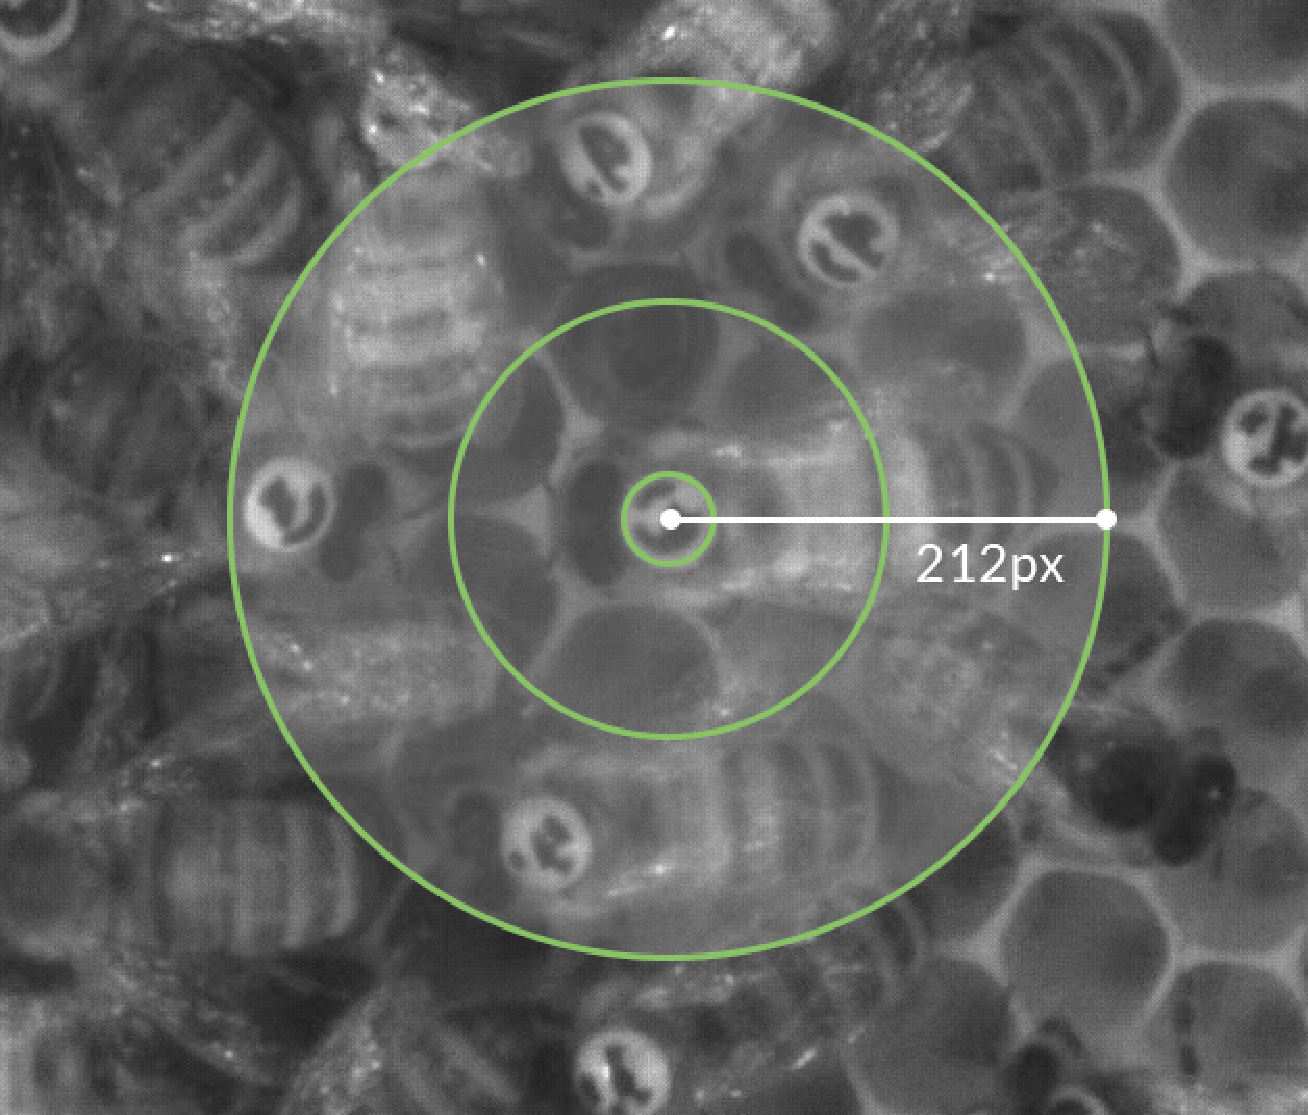
\includegraphics[width=\textwidth]{Figures/radius}
		\caption[Contact Radius]{Contact Radius}
		\label{fig:radius}
	\end{subfigure}
	\begin{subfigure}[b]{0.4\textwidth}
		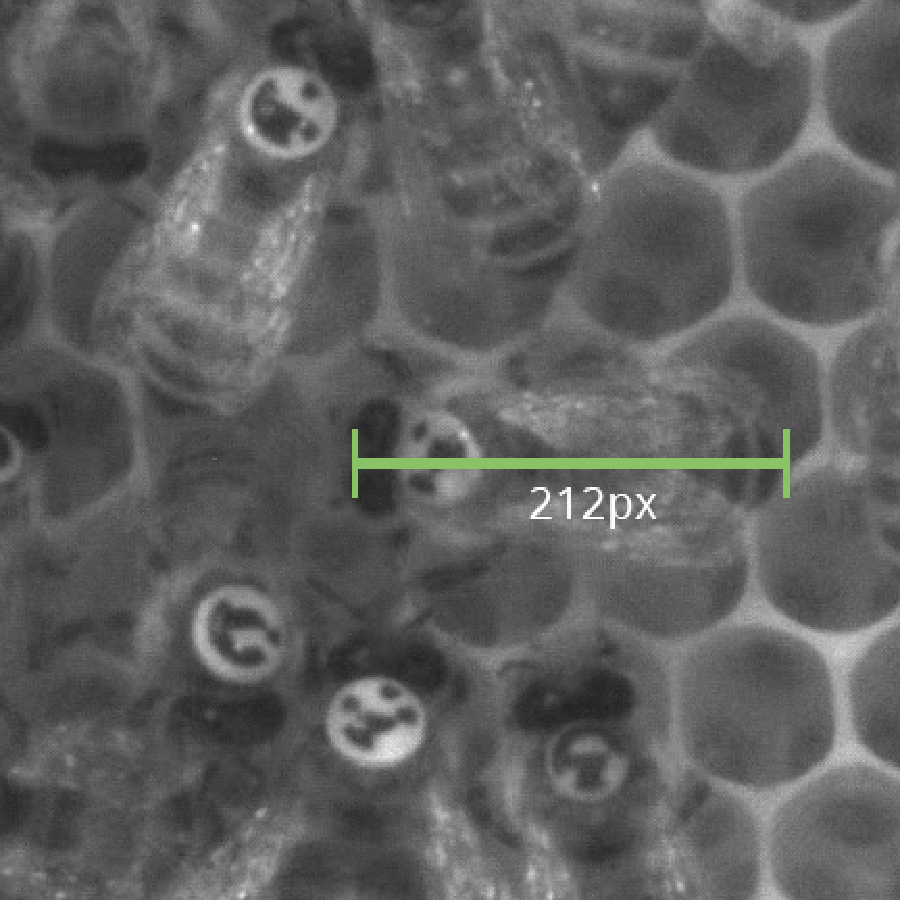
\includegraphics[width=\textwidth]{Figures/sizeTagBee}
		\caption[Bee and Tag Size]{Bee Length}
		\label{fig:size}
	\end{subfigure}
	\caption{Distance Between Bees: A length of a bee is chosen as the maximal  distance between bees.}
	\label{fig:contactRadius}
\end{figure}

\clearpage